\begin{figure}[h!]
\centering
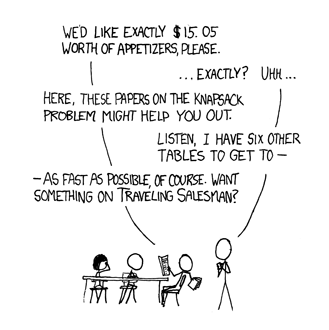
\includegraphics[height = 8cm]{../images/np_complete.png}
\end{figure}

 Parmi les problèmes d'optimisation, on distingue le cas des problèmes
 NP-difficiles. Ici, nous passerons en revue un ensemble de techniques
 exactes et approchées pour la résolution de ces derniers.

\begin{itemize}
  \item problèmes d'optimisation 
  \begin{itemize}
    \item[] $\nearrow$ problèmes faciles
    \item[] $\searrow$ \fbox{problèmes NP-difficiles}
  \end{itemize}
	\item méthodes exactes 
	\begin{itemize}
		\item[] $\nearrow$ programmation dynamique
		\item[] $\searrow$ branch and bound
	\end{itemize}
	\item méthodes approchées
	\begin{itemize}
		\item[] $\longrightarrow$ algorithmes d'approximation
	\end{itemize}
\end{itemize}

Nous implémenterons aussi certains algorithmes afin de mesurer
empiriquement leurs performances, et de comparer ce résultat à la
complexité théorique.

\subsection{Programmation dynamique}
La programmation dynamique permet de trouver la solution optimale d'un
problème en combinant les solutions optimales de sous-problèmes de ce
problème. Ces résultats intermédiaires sont sauvegardés, souvent sous
forme matricielle, ce qui permet d'éviter de répéter des calculs
inutilement.

Prenons par exemple le calcul du $n^{i\grave{e}me}$ nombre de la suite
de Fibonacci :

\begin{equation}
fibonacci(n) = 
\begin{cases}
1 \text{ si } n \leq 1; \\
fibonacci(n-2) + fibonacci(n-1) \text{ sinon};\\
\end{cases}
\end{equation}

Programmer une simple récursion nous fera calculer plusieurs fois les
mêmes résultats intermédiaires, c'est pourquoi il serait mieux de les
stocker dans un tableau. Évidemment nous sacrifions en mémoire ce que
nous gagnons en temps de calcul.


\subsection{Branch and Bound}
Un algorithme dit de Branch and Bound, ou Séparation et Évaluation en Français, se définit à partir de trois sous-stratégies :

\begin{itemize}
\item stratégie de \textbf{branchement},
\item stratégie d'\textbf{évaluation},
\item stratégie d'\textbf{exploration}.
\end{itemize}

À chaque itération, la séparation nous permet de diviser l'espace des
solutions possibles en plusieurs sous ensembles, ou branches,
l'évaluation permet d'éliminer certains de ceux-ci, et l'exploration
définit comment explorer ceux qui restent. Notons que nous devons
partir d'une solution initiale, souvent obtenue en utilisant une
méta-heuristique, afin de définir une première borne qui servira pour
l'élimination de branches.

Contrairement à la programmation dynamique nous pouvons avoir une
solution très rapidement ou très lentement selon l'instance.

\subsection{Algorithmes d'approximation}
Les algorithmes d'approximation permettant d'apporter en temps
polynomial une solution non-optimale à un problème
NP-difficile. Parfois nous pouvons définir une borne d'approximation
qui garantit la solution par rapport à l'optimal (classe
APX\footnote{APX : approximable. }) ou même paramétrer l'algorithme
pour avoir une solution plus ou moins bonne selon le temps de calcul
(classes PTAS et FPTAS\footnote{ PTAS et FPTAS : (fully)
  polynomial-time approximation scheme}).
